\newpage
\section{Consuntivo e Preventivo a finire}

In questo capitolo viene effettuato un confronto fra le ore ed il costo preventivati con quelli riscontrati effettivamente durante i periodi del ciclo di sviluppo.
Viene poi analizzato e riportato il bilancio che potrà essere:
\begin{itemize}
	\item \textbf{positivo}: se il consuntivo risulta inferiore o equivalente al preventivo;
	\item \textbf{negativo}: se il consuntivo risulta superiore al preventivo.
\end{itemize}

\subsection{Analisi dei requisiti}
\subsubsection{Consuntivo}
Di seguito è riportata la tabella riassuntiva per il consuntivo del primo periodo
\begin{table}[h!]
	\centerline{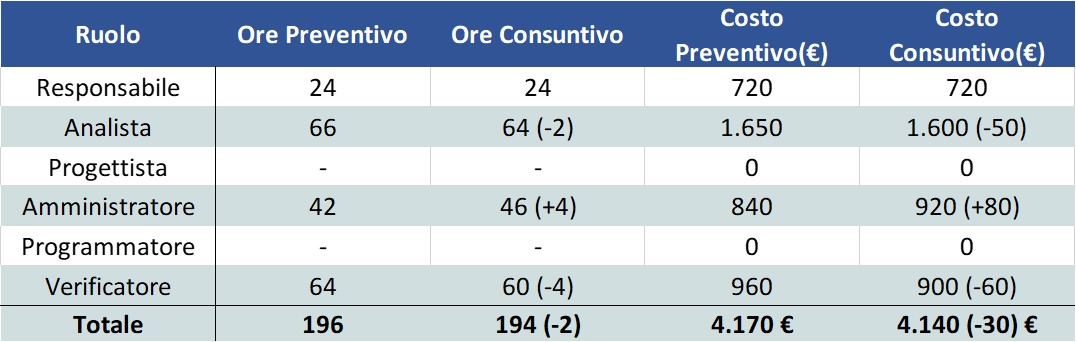
\includegraphics[scale=0.55]{img/Preventivo/AnalisiRequisitiConsuntivo.jpg}}
	\caption{Consuntivo: Analisi dei requisiti}
\end{table}

\subsubsection{Conclusioni}
In conclusione, durante questo primo periodo non ci sono state grandi discordanze rispetto a quanto pianificato. È possibile visionare i problemi riscontrati nell'\hyperref[RiscontroRischi]{Appendice A} e notare come essi abbiano influito sullo scostamento delle ore totali preventivate e di conseguenza sul costo. Si è inoltre rivelato necessario un impegno minore da parte dei \vers{} rispetto a quanto preventivato.\\
Questi fattori hanno favorito un risparmio rispetto al costo inizialmente preventivato pari a \EUR{30} e quindi il bilancio di questo primo periodo risulta positivo.
